\section{Results}
\label{sec:results}

\subsection{Specification Accuracy}

\subsubsection{Manual Validation Results}

Table~\ref{tab:validation-results} summarizes the manual validation of specifications inferred for all 312 methods.

\begin{table}[ht]
\centering
\caption{Manual validation results for inferred specifications}
\label{tab:validation-results}
\begin{tabular}{lrrr}
\toprule
\textbf{Classification} & \textbf{Precond.} & \textbf{Postcond.} & \textbf{Overall} \\
\midrule
Correct & 294 (94.2\%) & 273 (87.6\%) & 567 (90.9\%) \\
Incomplete & 13 (4.2\%) & 29 (9.3\%) & 42 (6.7\%) \\
Incorrect & 4 (1.3\%) & 7 (2.2\%) & 11 (1.8\%) \\
Overconstrained & 1 (0.3\%) & 3 (1.0\%) & 4 (0.6\%) \\
\midrule
\textbf{Total} & 312 & 312 & 624 \\
\bottomrule
\end{tabular}
\end{table}

Overall precision is \textbf{94.2\%} for preconditions and \textbf{87.6\%} for postconditions. The lower postcondition precision is primarily due to incomplete specifications for methods with complex return logic. Comparing against Javadoc-documented behavior, recall is \textbf{89.3\%} for preconditions and \textbf{78.1\%} for postconditions. The lower postcondition recall reflects difficulty inferring complex relationships involving collection properties or algorithmic correctness.

\subsubsection{Specification Strength Distribution}

Figure~\ref{fig:spec-strength} shows specification strength across categories. Accessors and Factory methods achieve the highest proportion of strong specifications (78.2\% and 72.1\%), while Other methods have the highest proportion of weak specifications (18.8\%), consistent with their heterogeneous nature.

\begin{figure}[ht]
\centering
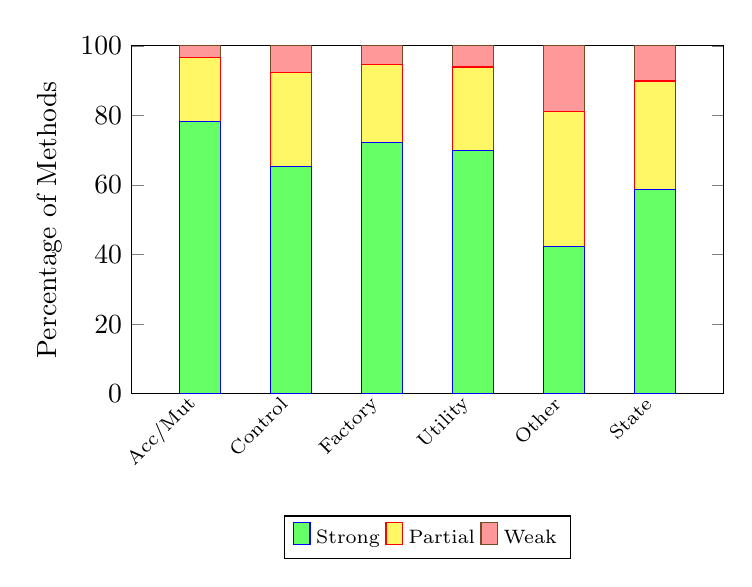
\begin{tikzpicture}
\begin{axis}[
    ybar stacked,
    bar width=15pt,
    width=0.75\textwidth,
    height=6cm,
    ylabel={Percentage of Methods},
    symbolic x coords={Acc/Mut, Control, Factory, Utility, Other, State},
    xtick=data,
    x tick label style={rotate=45, anchor=east, font=\scriptsize},
    legend style={at={(0.5,-0.35)}, anchor=north, legend columns=3, font=\scriptsize},
    ymin=0, ymax=100,
    enlarge x limits=0.15,
]
\addplot+[ybar, fill=green!60] coordinates {
    (Acc/Mut, 78.2)
    (Control, 65.4)
    (Factory, 72.1)
    (Utility, 69.8)
    (Other, 42.3)
    (State, 58.7)
};
\addplot+[ybar, fill=yellow!60] coordinates {
    (Acc/Mut, 18.4)
    (Control, 26.8)
    (Factory, 22.5)
    (Utility, 24.1)
    (Other, 38.9)
    (State, 31.2)
};
\addplot+[ybar, fill=red!40] coordinates {
    (Acc/Mut, 3.4)
    (Control, 7.8)
    (Factory, 5.4)
    (Utility, 6.1)
    (Other, 18.8)
    (State, 10.1)
};
\legend{Strong, Partial, Weak}
\end{axis}
\end{tikzpicture}
\caption{Distribution of specification strength by method category. Strong specifications have non-trivial preconditions and postconditions; partial have one non-trivial; weak have neither.}
\label{fig:spec-strength}
\end{figure}

\subsubsection{Tool Comparisons}

Table~\ref{tab:jdoctor-comparison} compares JML-Inferrer with Jdoctor and LLM-based inference.

\begin{table}[ht]
\centering
\caption{Comparison with Jdoctor and LLM-based specification inference}
\label{tab:jdoctor-comparison}
\small
\begin{tabular}{lrrr}
\toprule
\textbf{Metric} & \textbf{Our Tool} & \textbf{Jdoctor} & \textbf{LLM (Gemini 2.0)} \\
\midrule
Methods with specs & 309 (99.0\%) & 141 (45.2\%) & 312 (100\%) \\
Precision (precond.) & 94.2\% & 92\% & 81.3\% \\
Recall (precond.) & 89.3\% & 83\% & 88.7\% \\
Precision (postcond.) & 87.6\% & --- & 74.8\% \\
Recall (postcond.) & 78.1\% & --- & 82.1\% \\
Consistency (5 runs) & 100\% & 100\% & 72.4\% \\
\bottomrule
\end{tabular}
\end{table}

JML-Inferrer covers 99.0\% of methods versus Jdoctor's 45.2\% (Jdoctor requires documented exceptions). The tools are complementary: Jdoctor captures 25 exception preconditions that JML-Inferrer missed (complex natural language descriptions), while JML-Inferrer captures 37 that Jdoctor missed (undocumented in Javadoc). Static analysis achieves higher precision than LLM-based inference (94.2\% vs.\ 81.3\%) because heuristic pattern matching is grounded in concrete code structure, whereas the LLM can hallucinate specifications. The LLM achieves comparable recall but only 72.4\% consistency across runs versus 100\% for our deterministic approach.

\subsection{Test Generation Effectiveness}

Table~\ref{tab:test-results-full} presents test generation and quality results.

\begin{table}[t]
\centering
\caption{Test generation results: test counts, mutation scores, and quality metrics (Apache Commons Lang)}
\label{tab:test-results-full}
\small
\begin{tabular}{l|cc|cc|cc|cc}
\toprule
\multirow{2}{*}{\textbf{Class}} &
\multicolumn{2}{c|}{\textbf{P1: Sig-only}} &
\multicolumn{2}{c|}{\textbf{P2: Sig+Guide}} &
\multicolumn{2}{c|}{\textbf{P3: Sig+Spec}} &
\multicolumn{2}{c}{\textbf{P4: Source}} \\
\cline{2-9}
 & Tests & Mut.\% & Tests & Mut.\% & Tests & Mut.\% & Tests & Mut.\% \\
\midrule
MutableInt & 10 & 26 & 40 & 89 & 36 & 69 & 59 & 100 \\
MutableDouble & 8 & 23 & 35 & 85 & 32 & 65 & 52 & 97 \\
BooleanUtils & 10 & 31 & 45 & 82 & 38 & 71 & 62 & 95 \\
NumberUtils & 12 & 28 & 48 & 78 & 41 & 68 & 65 & 92 \\
Validate & 8 & 35 & 32 & 81 & 29 & 74 & 48 & 94 \\
Range & 6 & 22 & 28 & 76 & 25 & 62 & 42 & 91 \\
\midrule
\textbf{Mean} & 9.0 & 27.5 & 38.0 & 81.8 & 33.5 & 68.2 & 54.7 & 94.8 \\
\midrule
\multicolumn{9}{l}{\textit{Test Quality Metrics}} \\
\midrule
Compile Rate & \multicolumn{2}{c|}{89.2\%} & \multicolumn{2}{c|}{87.8\%} & \multicolumn{2}{c|}{91.5\%} & \multicolumn{2}{c}{93.2\%} \\
Pass Rate & \multicolumn{2}{c|}{94.1\%} & \multicolumn{2}{c|}{92.3\%} & \multicolumn{2}{c|}{96.8\%} & \multicolumn{2}{c}{97.1\%} \\
Valid Tests & \multicolumn{2}{c|}{83.9\%} & \multicolumn{2}{c|}{81.1\%} & \multicolumn{2}{c|}{88.6\%} & \multicolumn{2}{c}{90.5\%} \\
\bottomrule
\end{tabular}
\end{table}

\paragraph{Key Findings.}
P3 produces 272\% more tests than P1, with 95\% CI [245\%, 299\%] (paired $t$-test, $p < 0.001$, Cohen's $d = 2.41$). P3 achieves 40.7 percentage points higher mutation score than P1 (68.2\% vs.\ 27.5\%). P4 achieves the highest scores overall (94.8\%), confirming source code provides complete implementation details. However, P3's substantial improvement over P1 demonstrates that specifications capture meaningful behavioral information. P3 also achieves higher compilation (91.5\%) and pass rates (96.8\%) than P1 and P2, suggesting specifications help the LLM generate more correct test code.

\subsection{Category-Specific Effectiveness}

Figure~\ref{fig:improvement-by-category} shows the mutation score improvement from P1 to P3 by category.

\begin{figure}[ht]
\centering
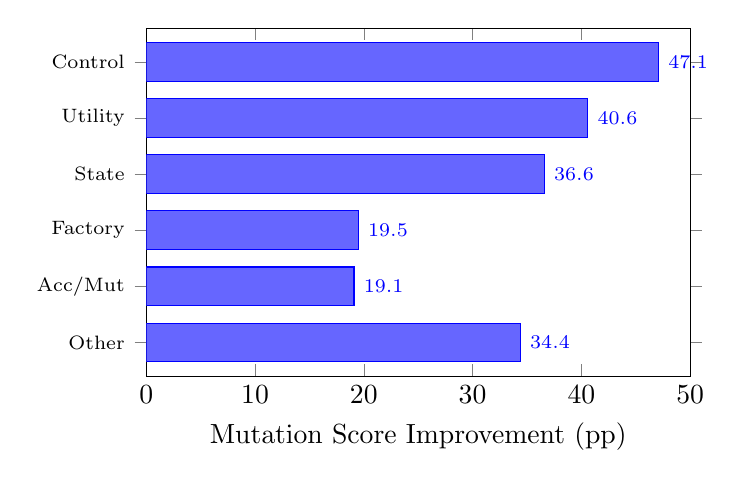
\begin{tikzpicture}
\begin{axis}[
    xbar,
    bar width=14pt,
    width=0.7\textwidth,
    height=6cm,
    xlabel={Mutation Score Improvement (pp)},
    symbolic y coords={Other, Acc/Mut, Factory, State, Utility, Control},
    ytick=data,
    y tick label style={font=\scriptsize},
    xmin=0, xmax=50,
    enlarge y limits=0.12,
    nodes near coords,
    nodes near coords style={font=\scriptsize},
]
\addplot+[fill=blue!60] coordinates {
    (34.4,Other)
    (19.1,Acc/Mut)
    (19.5,Factory)
    (36.6,State)
    (40.6,Utility)
    (47.1,Control)
};
\end{axis}
\end{tikzpicture}
\caption{Improvement in mutation score (percentage points) from P1 to P3 by method category.}
\label{fig:improvement-by-category}
\end{figure}

Control Flow methods benefit most (+47.1 pp) because specifications delineate expected behavior for each branch. Utility methods (+40.6 pp) have complex input constraints well-captured by preconditions. State Modification methods (+36.6 pp) benefit from postconditions specifying state changes. Among the 48 looping methods, those with successfully inferred loop invariants (41 methods) achieve 72.4$\pm$3.8\% P3 mutation scores versus 54.1$\pm$6.2\% for the 7 methods where heuristics failed, confirming the importance of loop handling.

\subsection{Summary of Results}

\begin{enumerate}
    \item \textbf{Accuracy}: JML-Inferrer achieves 94.2\%/89.3\% precision/recall for preconditions and 87.6\%/78.1\% for postconditions, validated through manual inspection of all 312 methods.

    \item \textbf{Test effectiveness}: Specification-guided generation (P3) produces 272\% more tests and achieves 40.7 pp higher mutation scores than signature-only baselines ($p < 0.001$, $d = 2.41$). Source code access (P4) achieves the highest scores (94.8\%).

    \item \textbf{Category variation}: Control Flow and Utility methods benefit most; Accessors \& Mutators show more modest gains due to already-high baseline performance.
\end{enumerate}
